\section*{Appendix B}
\label{sec:var_overlap}
We use the DGP described in Section~\ref{dgp1} with 2 relevant continuous covariates and no irrelevant covariates for both the coverage and the limited overlap experiments. Further, we set the parameters to the DGP as follows:
$\mu = 1$, $\Sigma = 1.5$, $\phi=0.5$, $\sigma = 20$ and $c = 2$.
\subsection*{Coverage Study}
% WRITE ABOUT VARIANCE ESTIMATION PROCEDURE (MAYBE USE SOME OF THE TEXT FROM RESULTS SECTION).
We selected 9 reference points in a grid from the covariate space as shown in Figure~\ref{fig:Coverage}(b) and conducted an experiment that considered these reference points, over 100 repetitions. We compared coverage for CATEs estimated using MALTS for different values of variance, ranging from 1.0 to 4.0, for noise term $\epsilon_0$ and $\epsilon_1$ in the potential outcomes function. 

Variance estimation is notoriously hard in matching problems, even for overall quantities such as the average treatment effect \citep{doi:10.1111/j.1468-0262.2006.00655.x} and is part of ongoing work for the authors. We consider both the conservative variance estimator \citep{wang2017flame} and estimators that sacrifice some interpretability for better coverage. We consider the CATEs estimated using MALTS and study how well an uninterpretable method can predict those estimates. We use the predictive variance from gradient boosting regressor, from Gaussian Process regression and from Bayesian Ridge regression on the covariates and estimated average CATEs to quantify variance of each CATE estimate.

\begin{figure}
    \centering
    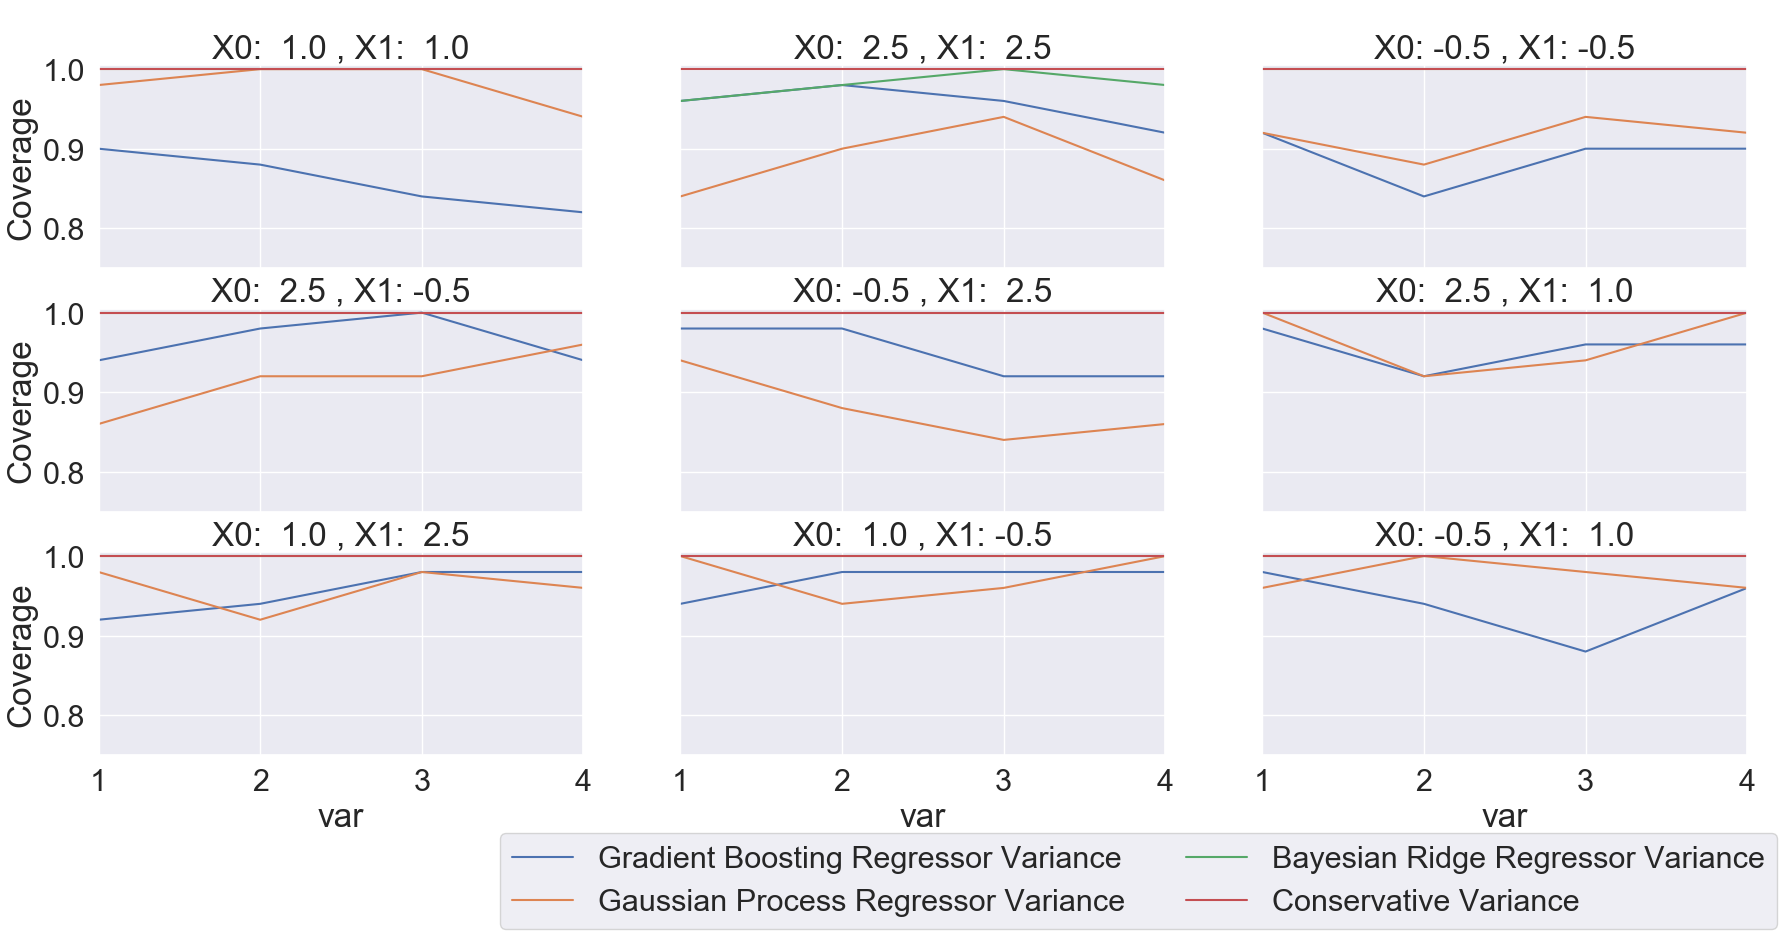
\includegraphics[width=\textwidth]{Figures/coverage.png}\\(a)\\
    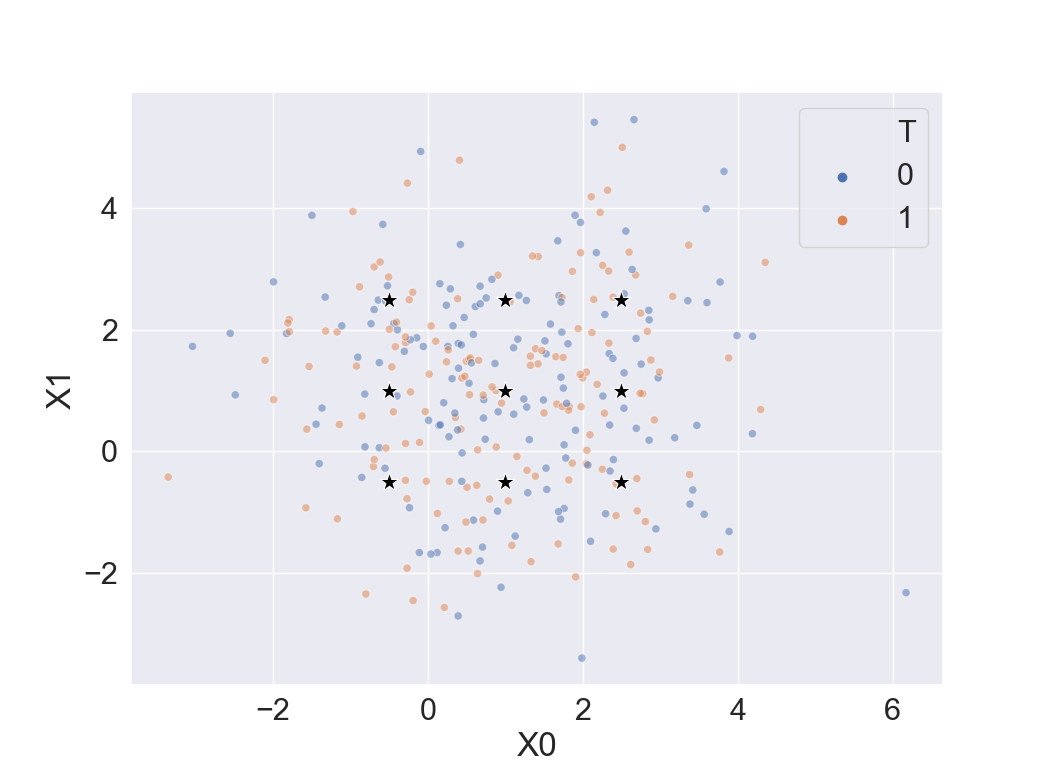
\includegraphics[width=0.7\textwidth]{Figures/coverage_space.png}\\(b)
    \caption{(a) Coverage of 95 percent confidence interval for 9 points: (1.0,1.0), (2.5,2.5), (-0.5,-0.5), (2.5,-0.5), (-0.5,2.5), (4.0,4.0), (-3.0,-3.0), (4.0,-3.0) and (-3.0,4.0). (b) Covariate space showing positions of 9 points-of-interest as black-stars, with other points color-coded according to their treatment assignments.}
    \label{fig:Coverage}
\end{figure}

Based on Figure~\ref{fig:Coverage}(a), the coverage for each the nine points of interest is between 0.9 and 1 for most of the values of variances using either of the three variance estimation approaches.

\subsection*{Limited Overlap and Performance}
We performed experiments on the overlap by changing the variance of the noise term $\epsilon_t$ in the treatment assignment equation of the DGP and measured CATE estimation error for MALTS for each of the scenarios. A lower variance leads to small overlap, i.e., large standardized difference of means, whereas large variance means small standardized difference of means and high overlap.
Figure~\ref{fig:overlap}(a) shows the performance of MALTS in predicting CATEs for 500 units in  2 dimensions generated with different levels of overlap (represented as standardized difference of means). Figure~\ref{fig:overlap}(b) shows four datasets generated with different level of overlap between the treated and control groups. MALTS performs reasonably well even under limited overlap. As expected, performance deteriorates as overlap decreases.
    \begin{figure}
        \centering
        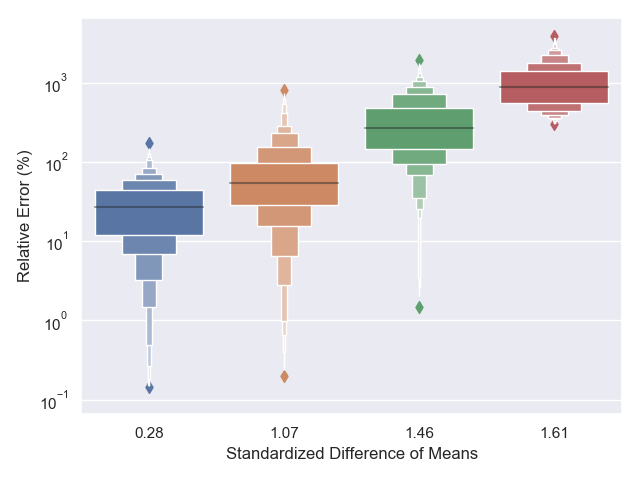
\includegraphics[width = 0.7\textwidth]{Figures/overlap.png}\\
        (a)\\
        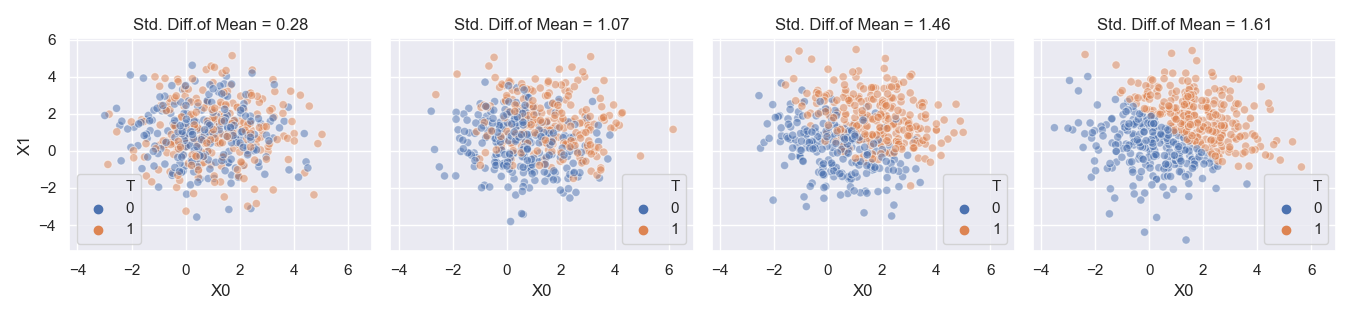
\includegraphics[width = \textwidth]{Figures/overlap_space.png}\\
        (b)
        \caption{(a) Comparison of MALTS performance measured as relative error for CATE estimation under different level of overlap measured as standardized difference of means. (b) The plots show the distribution of data generated for assessing the performance of MALTS under limited overlap.}
        \label{fig:overlap}
    \end{figure}
    
\subsection*{Sensitivity Analysis}
We performed a \textit{sensitivity analysis} of MALTS on a data generative setup with a constant unit treatment effect, two observed relevant covariates, and an unobserved confounder affecting the probability distributions of outcome as well as the choice of treatment. The unobserved confounder has a linear relationship with the outcome with the value of the coefficient equal to the ``sensitivity parameter of the Outcome'' ($\gamma_Y$) and the choice of treatment with the value of the coefficient equal to the ``sensitivity parameter of the Treatment'' ($\gamma_T$).
\begin{eqnarray*}
    && x_{i,1},x_{i,2}, u_i \overset{iid}{\sim} \mathcal{N}(0,1)\\
    && \epsilon_0, \epsilon_1 \overset{iid}{\sim} \mathcal{N}(0,1)\\
    y_i^{(0)} &=& x_{i,1} + x_{i,2} + \gamma_Y u_i + \epsilon_0 \\
    y_i^{(1)} &=& x_{i,1} + x_{i,2} + \gamma_Y u_i + 1 + \epsilon_1 \\
    t_i &=& \text{Bernoulli}\left(\text{expit}\left( x_{i,1} + x_{i,2} + \gamma_T u_i - 2 \right) \right)\\
    y_i &=& t_i(y_i^{(1)} + (1-t_i)(y_i^{(0)}
\end{eqnarray*}
Figure~\ref{fig:sensitivity} shows the contour plot of ATE estimates produced by MALTS as we change the sensitivity parameters in the data generative process. Here, the true ATE equals to 1.
    \begin{figure}
        \centering
        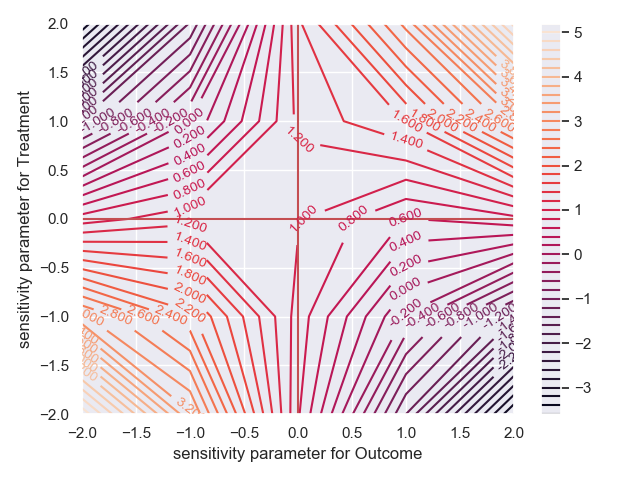
\includegraphics[width=0.85\textwidth]{Figures/sensitivity_analysis.png}
        \caption{Sensitivity analysis contour plot of the ATE estimation using MALTS}
        \label{fig:sensitivity}
    \end{figure}
